\section{Preliminary}\label{sec:preliminary}
Before introducing the process of CNN training, we first claim the symbols used in this section in Table~\ref{tab:symbol}.

% Table generated by Excel2LaTeX from sheet 'Sheet1'
\begin{table}[htbp]
    \centering
    \caption{Symbol used to describe training}
      \begin{tabular}{lp{0.7\columnwidth}} \hline
      Symbol   & Description \\ \hline
      $x$      & network input \\
      $y_i$    & output of layer i \\
      $f_i$    & function of layer I, can be 2d convolution, matrix vector multiplication, ReLU, pooling, etc. \\
      $W_i$    & weights of layer i \\
      $\alpha$ & learning rate \\
      $E$      & error of the network output \\ \hline
      \end{tabular}%
    \label{tab:symbol}%
  \end{table}%

\subsection{Training Flow of CNN}
Training of neural network is usually done with stochastic gradient descent. An example flow is shown in Figure~\ref{fig:train_prelim} The training process consists of two alternate phases: forward phase(FP) and back-propagation(BP). The forward phase randomly select a batch of training inputs and calculates their inference result with the current model. The back-propagation phase calculates the gradient of error to the weights in each layer according to the chain rule and update the weights by gradient descent. We further separate this phase into 2 phases: error back-propagation (EB) phase calculates the gradient of error, $\partial E/\partial y_i$ to the output of each layer; weight gradient (WG) phase calculates the gradient of weights $\partial E/\partial W_i$ in each layer and update the weights. 

One trains a CNN by iteratively conduct FP and BP until the weights converge. In each iteration, a batch of inputs are sent to the network and the corresponding gradients are added together to update the weights.

\begin{figure}[t]
  \centering
  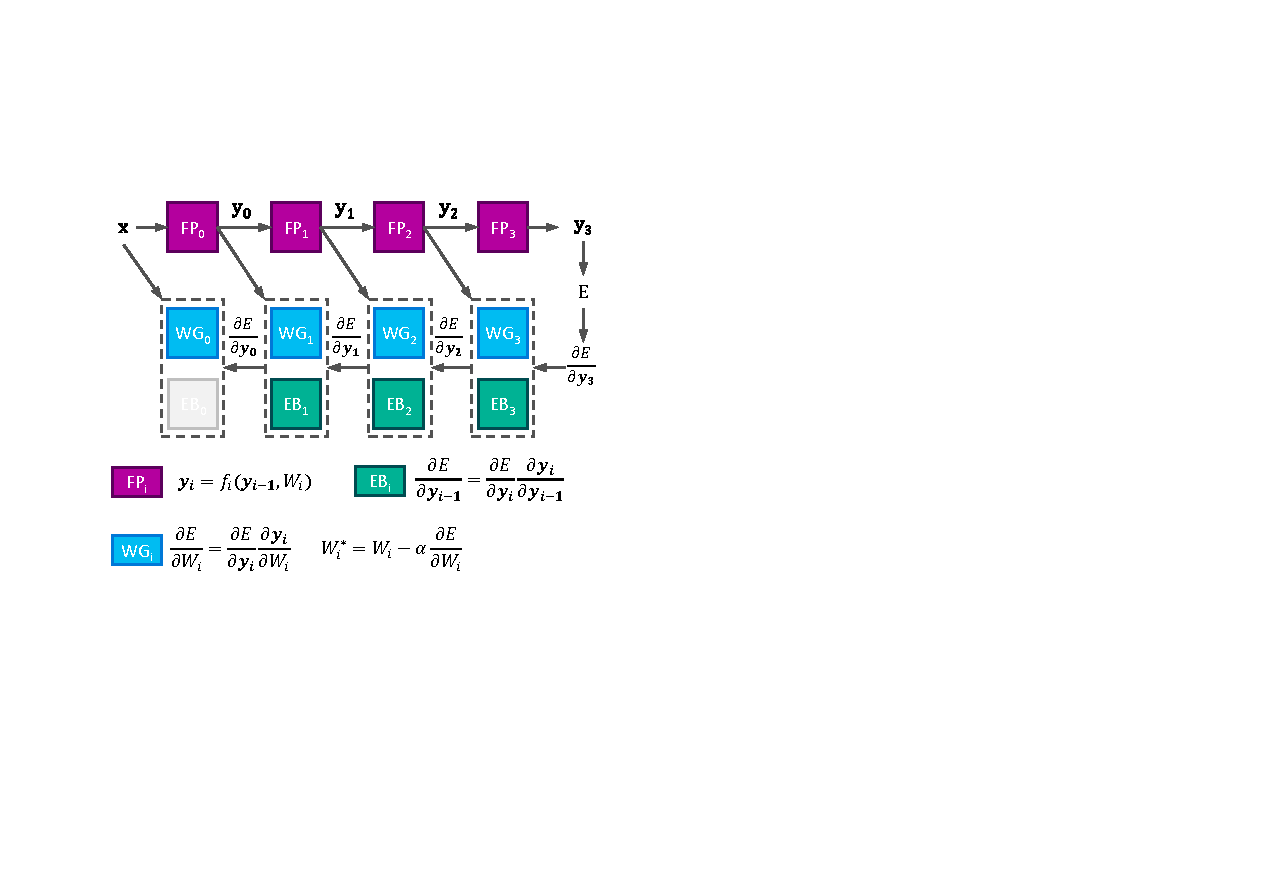
\includegraphics[width=1\columnwidth]{figures/train_prelim.pdf}
  \caption{An example flow of training a 4 layer neural network. $f_i$ and $W_i$ denote the function and weight of each layer respectively.}
  \label{fig:train_prelim}
\end{figure}

\subsection{Computation Pattern for BP}
The computation pattern for training CNN is similar to inference. For convolution layers, EB phase conducts convolution on the output error with the rotated kernels as shown in equation~\ref{eqt:eb_conv}, where M and N denote the number of input and output channel. WG phase conducts the convolution on the input feature map with the output error as shown in equation~\ref{eqt:wg_conv}.

\begin{equation}\label{eqt:eb_conv}
  \fpartial{E}{\mathbf{y_{i-1}}(m)} = \sum\limits_{n=0}^{N-1}\text{conv2d}(\fpartial{E}{\mathbf{y_i}}, rot180(\mathbf{W_i}(m,n)))
\end{equation}

\begin{equation}\label{eqt:wg_conv}
  \fpartial{E}{\mathbf{W_i}(m, n)} = \text{conv2d}(\mathbf{y_{i-1}}(m), \fpartial{E}{\mathbf{y_i}(n)})
\end{equation}

For fully connected layers, the inference phase is simply matrix vector multiplication. So the EB and WG phases can be expressed in equation~\ref{eqt:eb_fc} and \ref{eqt:wg_fc} respectively.

\begin{equation}\label{eqt:eb_fc}
  \fpartial{E}{\mathbf{y_{i-1}}} = \mathbf{W_i}^\top \fpartial{E}{\mathbf{y_i}}
\end{equation}

\begin{equation}\label{eqt:wg_fc}
  \fpartial{E}{\mathbf{W_i}} = \left( \fpartial{E}{\mathbf{y_i}} \right)^\top \mathbf{y_{i-1}} 
\end{equation}

